%\documentclass[a4paper,10pt]{article}
\documentclass[10pt]{article}
\usepackage[utf8]{inputenc}
\usepackage{xspace}
\usepackage{url}
\usepackage{graphicx,graphics} 
\usepackage{color}
\usepackage{amsmath}
\usepackage{amsfonts}
\usepackage{amssymb}
\usepackage{caption}
\usepackage{amsthm}
\usepackage{algorithm}
\usepackage{algorithmic}
\usepackage{longtable}
\usepackage{complexity}
\usepackage{tkz-graph}
\usepackage{float}
\usepackage{tabularx}
\usepackage{setspace}
\usepackage{icomma}
\renewcommand{\algorithmicrequire}{\textbf{Input:}}
\renewcommand{\algorithmicensure}{\textbf{Output:}}
\usepackage{authblk}
\usepackage[colorlinks=true,breaklinks=true,linkcolor=blue]{hyperref}

% sr
\newcommand\rmatching{${\cal R}$-matching\xspace}
\newcommand\mdelay{$\cal M$-delay\xspace}
\newcommand\matchedgraph{{\bf matched graph}}
\newtheorem{proposition}{Proposition}
\newtheorem{theorem}{Theorem}

\setlength{\parskip}{1ex} % Espace entre les paragraphes

\newtheorem{fact}{Fact}
\newtheorem{lemma}[theorem]{Lemma}
\newtheorem{definition}{Definition}
\newtheorem{corollary}{Corollary}

% \renewcommand{\thefootnote}{\*}

\newcommand{\todo}[1]{{\color{red} TODO: {#1}}}
\newcommand\pazl{\textsc{pazl}\xspace}
\newcommand\pall{\textsc{PALL}\xspace}
\newcommand\spazl{\textsc{spazl}\xspace}
\newcommand\spall{\textsc{SPALL}\xspace}
\newcommand\bra{\textsc{bra}\xspace}
\DeclareMathOperator{\pdv}{pdv}
\newcommand\pra{\textsc{pra}\xspace}
\newcommand\minpra{\textsc{min-pra}\xspace}
%opening
\title{Deterministic Scheduling of Periodic Messages for Cloud RAN}
 

\author[1]{Dominique Barth}
\author[1,2]{Ma\"el Guiraud}
% \author[1]{Christian Cad\'er\'e}
 \author[2]{Brice Leclerc}
 \author[2]{Olivier Marc\'e}
\author[1]{Yann Strozecki}
\affil[1]{David Laboratory, UVSQ}
\affil[2]{Nokia Bell Labs France}

\begin{document}

\maketitle

\section{General model and Problems}\label{sec:def}

We use the notation $[n]$ to denote the interval of $n$ integers $\{0,\dots,n-1\}$.

  \subsection{Discrete time model}
  In the model presented here, the time is discrete. The unit of time  is called a {\bf tic}. This is the time needed to transmit an atomic data of size $Q$ over the fastest link of the network. Since the speed of the links on the network can be different, the number of tics needed to transmit an atomic data through a link can be different depending on the link. In order to consider only integers, the fastest link of the network can be virtual if there is no link of speed equal to the least common multiple of the speeds of all links in the network. We denote by $s_{(u,v)}$ the speed of the link $(u,v)$, and ${\cal S}$ the set of speed of all the links. The number of tics needed to send an atomic data of size $Q$ on a link $(u,v)$ is thus equal to $\frac{LCM({\cal S})}{s_{(u,v)}}$ tics, where $LCM({\cal S})$ is the Least Common Multiple of the set {\cal S}. Figure~\ref{fig:datagram} illustrates this phenomenon.
  
  \begin{center}
  
  \begin{figure}
  \begin{minipage}[b]{0.50\linewidth}
  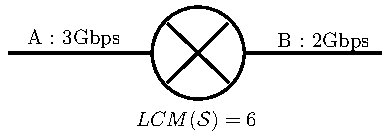
\includegraphics[width=0.8\textwidth]{links.pdf}
  \end{minipage}
\hfill
  \begin{minipage}[b]{0.50\linewidth}
    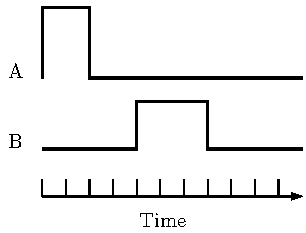
\includegraphics[width=0.8\textwidth]{chronotics.pdf}
  \end{minipage} 
  \caption{Different number of tics used to carry an atomic data of size $Q$}
  \label{fig:datagram}
 \end{figure}
 
    \end{center}
  \subsection{Network modeling}
  
The network is modeled as a directed graph $G=(V,A)$. The \textbf{sending tic} of a message in a vertex $u$ is the tic at which the beginning of this message is sent from $u$. Also, the \textbf{reception tic} of a message in a vertex $v$ is the tic at which the beginning of the message arrives in $v$.  Each arc  $(u,v)$ in $A$ is labeled by an integer weight $\Omega(u,v)$ which represents the number of tics elapsed between the sending tic of the message in $u$ and the reception tic of this message in $v$ using this arc. A {\bf route} $r$ in $G$ is a directed path, that is, a sequence of adjacent vertices $u_0, \ldots , u_{l}$, with $(u_i,u_{i+1}) \in A$.  The {\bf weight of a vertex} $u_i$ in a route $r=(u_0,\dots,u_l)$ is defined by $\lambda(u_i,r)= \sum\limits_{0 \leq j <i} \Omega(u_j, u_{j+1})$. It is the number of tics needed between the sending tic of a message in the first vertex of the route and the reception tic of this message at $u_i$. We also define $\lambda(u_0,r)=0$. The weight of the route $r$ is defined by $\lambda (r)= \lambda (u_l,r)$.
We denote by $\cal R$ a set of routes, the pair $(G,\cal R)$ is called a {\bf routed network} and represents our telecommunication network.
The first vertex of a route models an antenna (RRH) and the last one a data-center (BBU) which computes an answer to the messages sent by the antenna.

   \subsection{Messages dynamic}
	 
    %Time is discretized, hence the unit of all time values is a, the time needed to transmit a minimal unit of data over the network. \todo{parler des différents débits et de ce que ça change}. The weight of an arc is also expressed in tics, that is the time needed by a message to go through this arc.
    
        In the process we study, some {\bf datagrams} are sent on each route. The size $|d|$ of a datagram $d$ is an integer, and correspond to the number of atomic data needed to carry the information contained by the datagram. The number of tics needed by a node $u$ to emit the datagram through the link $(u,v)$ of speed $s_{(u,v)} = {\cal S}(u,v)$ is denoted $|d|_{(u,v)}$ and has for value $ |d| \times \frac{LCM({\cal S})}{s_{(u,v)}}$ . Once a datagram has been emitted, it cannot be fragmented during its travel in the network. Thus, due to the different speed of the links, when the beginning of a datagram $d$ arrives in a node $v$ of a route $r$, it might be delayed in the node to avoid the fragmentation of the datagram. The number of tics lost in the node is given by the function $b(d,v,r)$.\\
        \begin{lemma}
        If a datagram $d$ arrives at a node $v$ through the link $(u,v)$ of speed $s_i$, and must be sent back in the link $(v,w)$ of speed $s_j$, then $b(d,v,r)$ is equal to $ \max( 0, |d|_{(u,v)} - |d|_{(v,w)} )$ tics.
        \end{lemma}
        \begin{proof}
        We consider a buffer in the node $v$. If $t$ is the reception tic of the datagram $d$ in $v$, the last tic of the $d$ has reached the buffer  at date $t+|d|_{(u,v)}$. The node can start to emit immediatly after the reception of the first tic of the datagram, if it is possible. We want to choose the sending tic such that the datagram will not be fragmented. This mean that the buffer must contain enough data to fill a tic on the link $(v,w)$.\\
        
        If $s_i \geq s_j$, the buffer fills as fast or faster as it empties, thus, the datagram crosses the node without additional delay.\\
   
        If $s_i < s_j$, the buffer need to be filled a bit before the emission of the datagram, in order to send back the datagram without fragmentation. The last tic at which the node receive some data is $t+|d|_{(u,v)}$. Thus, the next tic ($t+|d|_{(u,v)}+1$), is the minimum date at which the node can send the end of the datagram on the link $(v,w)$. Since the node needs $|d|_{(v,w)}$ to completely send the datagram, it can start to emit at date $t+|d|_{(u,v)}+ 1 - |d|_{(v,w)}$. 
        \end{proof}
        
          Let $r=(u_0,\dots,u_l)$ be a route. In order to avoid the contention, one can choose to buffer a datagram $d$ in any node $u_i$ of the route. The function $l(d,u_i,r), i \in \{0,\ldots,l\}$ associate to each couple datagram-node of the route an integer. Those integers represent the buffering time of the datagram in each nodes of the route.
              
The \textbf{departure date} of a datagram $d$ on a route $r$, denoted by $\theta_r(d)$, is the sending tic of $d$ at node $u_0$, the first vertex of $r$. 
 Also, the \textbf{reception date} of this datagram $d$ at a vertex $u_i$ in $r$, i.e. the first tic at which the datagram sent at date $\theta_r(d)$ on $r$ reaches $u_i$, is $t(d,u_i,r) = \theta_r(d) + \lambda(u_i,r) + \sum_{k=0}^{i-1}( b(d,u_k,r) + l(d,u_k,r))$. In other words, the date at which a datagram reach a vertex $u_i$ correspond to the date of the emission of this datagram in the RRH, plus the physical delay of the links, plus the buffers induced by the physical constraints of the network, or determined by the logical solutions proposed.
   
        A {\bf stream} $St$ is a sequence of several datagrams. To each route of the routed network is associated a stream. The cardinal of a stream, denoted $\#St$ is the number of datagrams in the stream. Let us consider a stream $St_i$ on the route $r_i$, the datagrams $\{d_0,\ldots,d_{\#St_i-1}\}$ are sent in sequence from the first node of the route, that is : $\theta_{r_i}(d_0) < \theta_{r_i}(d_1) < \ldots < \theta_{r_i}(d_{\#St_i-1})$ .  \\
     % For each route, the size of a stream is $|St| = \sum_{i=0}^{{\#St-1}} |d_i|$ . The amount of data sent by an RRH to its BBU is the same, regardless of the route. Hence, we assume that this size is the same for all route, and we denote it by $\tau$. This means that for all routes $r$, $|St_r| = \tau$.
        
          
       Let us call $[t(St,u)]$ the set of tics used by a stream $St$ on a route $r$ in the arc $(u,v)$, that is $[t(St,u)] =  \bigcup_{i=0}^{\#St -1} \{t(d_i,u,r) + k \mid 0 \leq k < |d_i|_{(u,v)}\}$.
      Let $r_1$ and $r_2$ be two routes, on which two streams $St_1$ and $St_2$ are sent.
      We say that the two routes have a {\bf collision} if they share an arc $(u,v)$ and $[t(St_1,u)] \cap [t(St_2,u)] \neq \emptyset$.
      
      In the model presented here, the sending of the streams is \textbf{periodic}; during each period of $P$ slots, each datagram of the stream is sent at the same tic in the period.
            
  \begin{subsection}{Notion of jitter}
   We define by {\bf delay} of a datagram $d$ in a node $u_i$ of a route $r$, the time taken by the datagram to go from $u_0$, the first vertex of the route to $u_i$ through $r$.
 Thus, the delay of a datagram in the node $u_i$ is equal to $DL(d,u_i,r) =  t(d,u_i,r) - t(d,u_0,r) = \lambda(u_i,r) + \sum_{k=0}^{i-1}( b(d,u_k,r) + l(d,u_k,r))$.
This delay is composed of three factors:
\begin{enumerate}
\item $\lambda(u_i,r)$ : it is the weight of the route. This time is not alterable. 
\item  $\sum_{k=0}^{i-1} b(d,u_k,r)$ : those values correspond to some {\bf physical buffers } induced by the potential speedup or slowdown of the different links of the route used.
\item $\sum_{k=0}^{i-1} l(d,u_k,r)$: are the {\bf logical buffers}. Those buffers are chosen by some algorithmic solutions in order to control the traffic in every node, and thus avoid collisions.
\end{enumerate}

As a reminder, a stream $St$ is a sequence of datagram. Each period, the sequence of datagrams $\{d_0,\ldots,d_{\#St-1}\}$, is sent on a route. The sequence of datagram is the same in every period: the same number of datagram which are of the same size are sent at the same tic in the period. For instance if the sequence $\{d_0,\ldots,d_{\#St-1}\}$ is sent at the first period $0$ on the route r at times $\{\theta_r(d_0),\ldots,\theta_r(d_{\#St-1})\}$ then the datagrams $\{d_{\#St \times k},\ldots,d_{(\#St \times k)-1}\}$ will be send in the next period $k$ at times $\{\theta_r(d_{\#St \times k}),\ldots,\theta_r(d_{(\#St \times k)-1})\}$, with $\theta_r(d_i) = \theta_r(d_{i \times k}) \mod P, \forall i \in [0,\ldots,\#St-1]$. We say that all the datagrams $d_{i \times k}$, forall $k$ are associated. 

The {\bf packet delay variation ($\pdv$) }\cite{demichelis_ip_nodate} is the variation of the delay between two datagram in a same node of a route. In this model, we allow some datagrams to be buffered in some nodes of the route, thus, the $\pdv$ between $d_0$ and $d_i$ can be greater than $0$. Formally, we denote the packet delay variation between two datagrams $d_i$ and $d_j$ in a node $u$ on a route $r$ by $\pdv(d_i,d_j,u,r) = |DL(d_i,u,r) - DL(d_j,u,r) | \ge 0$. 

Note that the $\pdv$ between two associated datagrams is always equal to zero. Indeed, our periodic and deterministic process implies that all the associated  datagrams of a stream have the same behaviour, independantly of the period.


Let us introduce the notion of {\bf jitter} \cite{guillemin_peak_1992} , which is commonly used in statistical networks to define the variance of the packet delay variations in a node. In the case of a deterministic network, $\pdv$ is only due to the logical buffers, which are also deterministic. 

Thus, we can define the jitter in a deterministic point of view:
\begin{itemize}
\item The jitter of a datagram, is exactly equal to the sum of all the logical buffers applied to this packet.
\item The jitter of a stream, is the maximum of the jitters of the datagram composing the steam.
\end{itemize}

One can observe that our notion of jitter and $\pdv$ are the same, thus, to avoid confusion, we will always talk about $\pdv$. 

  \end{subsection}


      \begin{subsection}{Cloud-RAN context}
     
      In the context of cloud-RAN applications, we need to send a stream from an RRH $u$ to a BBU $v$ and then 
      we must send the answer from $v$ back to $u$. We say that a routed network $(G, {\cal R})$ is \textbf{symmetric} if the set of routes is partitioned into the sets $F$ of \textbf{forward routes} and $B$ of \textbf{backward routes}. There is a bijection $\rho$ between $F$ and $B$ such that for any forward route $r \in F$ with first vertex $u$ and last vertex $v$, the backward route $\rho(r) \in B$ has first vertex $v$ and last vertex $u$. In all practical cases the routes $r$ and $\rho(r)$ will be the same with the orientation of the arcs reversed, which corresponds to bidirectional links in \emph{full-duplex} networks, but we do not need to enforce this property.
      
     We now describe the process of the sending of a stream and of its answer. First, the datagrams of a stream $St_r$ are sent at $u$, through the route $r \in A$, at times $\{\theta_r(d_0),\ldots,\theta_r(d_{\#St_r-1}) \}$.
      Those datagrams are received by $v$, i.e., the last vertex of $r$ at times $\{t(d_0,v,r),\ldots,t(d_{\#St_r-1},v,r)\}$. 
     Once $v$ has received all the datagrams of a stream, the answer is computed and sent back in a stream $St_{\rho_r}$. Note that $\#St_{\rho_r}$ may be not equal to $\#St_r$, i.e. the answer is not necessarily under the same form as the initial stream. Then, the node $v$ send $St_{\rho_r}$ to  $u$ on the route $\rho_r$ at times $\{\theta_{\rho_r}(d_0),\ldots,\theta_{\rho_r}(d_{\#St_{\rho_r}-1}) \}$.
     

     Note that, in the process we describe, we do not take into account the computation time a BBU needs to deal with one message. It can be encoded in the weight of the last arc leading to the BBU and thus we do not need to consider it explicitly in our model. 

     \end{subsection}
     \begin{subsection}{Definition of measures to optimize}
          We define the {\bf full reception date} of a stream $St_r$ on a node $v$ through the link $(u,v)$ by $rt(St_r,v) =  \displaystyle \max_{i \in \{0,\ldots,\#St_r-1\}} ( t(d_i,v,r) + |d_i|_{(u,v)} )$. This is the time at which the end of the last datagram of the stream has reached vertex $v$. Recall that a BBU needs to completely receive a stream before sending the answer, that is $rt(S_r,v)  < \theta_{\rho_r}(d_0)$.
     

      The whole process time for a route $r$ is equal to $PT(r)= rt(St_{\rho_r},u) - \theta_r(d_0) $, where $u$ is the RRH.      
      In the process time, we count the time elapsed between the date the first tic of the stream is emitted and the date at which the last tic of the answer comes back. 
      
       We define the \textbf{full transmission time} of a routed network $TR(G,R) = \displaystyle \max_{i \in \{0,\ldots,n\}} rt(St_{\rho_i},u) - \displaystyle \min_{j \in \{0,\ldots,n\}} \theta_j(d_0)$, where $u$ is the first node of the route $i$. This is the time ellapsed between the sending of the first tic of the first stream, and the reception of the last tic of the last stream.
        
        
      Each route must respect a time limit that we call \emph{deadline}. To represent these deadlines, 
     we use a deadline function $d$, which maps to each route $r$ an integer such that $PT(r)$ must be less than $d(r)$.
  

        An {\bf assignment} of a routed network $(G,\cal R)$ is a function that associates to each datagram of each route its departure date and its buffers function l. In an assignment, \emph{no pair of routes has a collision}.
        
        
        
              We consider the following problems.
       \subsubsection{Unsychronized sending of streams} 
       
   
      \noindent {\bf Periodic Assignment for Low Latency (\pall)} 

      \noindent {\bf Input:}  A symmetric routed network $(G,{\cal R})$, the period $P$, a deadline function $d$ and a set of streams.
      
      \noindent {\bf Question:} does there exist an assignment $m$ of $(G,{\cal R})$ such that for all $r \in {\cal R}$, $PT(r) \leq d(r)$?
      \noindent {\bf Optimisation problem:} Minimize $\displaystyle \max_{r \in R} PT(r)$.
      
       We also define another problem, in which we does not allow the message to be buffered in the nodes.\\
          \noindent {\bf Periodic Assignment for Zero Latency (PAZL)} 

      \noindent {\bf Input:}  A symmetric routed network $(G,{\cal R})$, the period $P$, a deadline function $d$ and a set of streams.
      
      \noindent {\bf Question:} does there exist an assignment $m$ of $(G,{\cal R})$, in which $l(d,u,r) = 0$, for all $d,u,r$ such that for all $r \in {\cal R}$, $PT(r) \leq d(r)$?
      
    There is no optimisation problem for this problem, because if a solution exists, it is already optimal in terms of latency, since there are no buffers.


        \subsubsection{Synchronized sending of streams}
     
        In the C-RAN context, it appears that the antennas start to emit their stream at the same tic.
        In this case, we can assume that all streams starts to emit at tic $0$, thus $PT(r)= rt(St_{\rho_r},u)$.
        Also, we replace the deadline function by a maximal response time $Tmax$. We want $TR(G,{\cal R}) \leq Tmax$.
        
         Thus, we have the following variant of \pall:
       
       \noindent {\bf Periodic Assignment for Low Latency (\spall)} 

      \noindent {\bf Input:}  A symmetric routed network $(G,{\cal R})$, the period $P$, $Tmax$ and a set of streams.
      
      \noindent {\bf Question:} does there exist an assignment $m$ of $(G,{\cal R})$ such that $ TR(G,{\cal R}) \leq Tmax$ ?

      \noindent {\bf Optimisation problem:} Minimizing $TR(G,{\cal R})$.
    
     
    \begin{lemma}
   
    To solve the problem \spall in a star shaped network, it is not useful to take choose the departure date of the datagrams in the first vertex of the route. Choosing the sequence of the datagrams in the central arc in the forward way is enough.
     \label{lemma:spallorder}
     \end{lemma}
   \begin{proof}
    Since all the streams can be sent at date $0$, if there is a gap of $a$ tics in the forward period between two datagrams $d_1$ and $d_2$, this mean that the datagram $d_2$ could have been sent $a$ tics earlier from the first node of the route. In the case of this delay of $a$ tics is essential to avoid collisions in the backward period , the algorithms allowing will just add this delay $a$ on the datagram $d_2$ on the first node of the route backward.
   \end{proof}
\todo{réécrire en bien plus propre, c'est pour l'idée}
      
        
        \end{subsection}
     \begin{subsection}{\pall and \spall: some different problems}
     
     
Here, we show that on a given routed network, the optimal solution for \pall is not necessarily optimal for \spall and vice versa.
  Consider the following example, represented in fig.\ref{fig:pallpallexample}; a star shaped network in which two routes $r_1$ of first vertex $u_1$ and last vertex $v_1$ and $r_2$ of first vertex $u_2$ and last vertex $v_2$ shares the same arc $(c_s,c_t)$. Thus, there is two contention points on the routed network, one on the way forward on the arc $(c_s,c_t )$, and one on the way backward on the arc $(c_t,c_s)$.
  We consider that the weight of the arcs $(u_i,c_s)$ is the same for every route $i$. For simplicity, and wlog, we set this weight to $0$. Also, the weight of the central arc can be ignored.
  We set the weight on the arc $(c_t,v_1)$ to $\tau -1$ greater than the weight of the last arc $(c_t,v_2)$. For simplicity, we also consider that those weights are then equal to $\tau-1$ and $0$.
  We take a period of $4\tau$, which is large enough to not care about the periodicity..\\
  
We want to solve \spall on this routed network. Lemma~\ref{lemma:spallorder} explains that choosing the permutation of the datagrams is enough in the forward period. In order to avoid contention, and considering that the weight of the arcs $(u_i,c_s)$ is the same, one departure time must be equal to $0$ and the other one must be $\tau$. If we send the datagram of the route $2$ first, then  $\theta(r_1) = \tau$, and $\theta (r_2) = 0 $, $PT(r_1) = 3\tau-3$, $PT(r_2) = \tau -1$ and $TR(G,{\cal R}) =4\tau-3$. Let us check if we can do better.\newline

Since the route $1$ is much longer than the route $2$, it is natural to send the message on the route $1$ first. 
Thus, $\theta(r_1) = 0$, and $\theta (r_2) = \tau $.\newline
If we do not delay the datagrams, then $[t(d_1,c_t,\rho_{r_1})] = [2\tau -2;3\tau-3]$ and $[t(d_2,c_t,\rho_{r_2})] = [\tau;2\tau-1]$. This is not possible since there is a collision in the backward period at tics $2\tau-2$ and $2\tau-1$.
  Thus, there is two possibility: 
  \begin{enumerate}
                                                                                                                                                                                                                                                                                                                                                                                                                                               \item Adding some waiting time on the route 1; $w_1 = 2$. Thus $PT(r_1) = 3\tau-1$, $PT(r_2) = \tau -1$ and $TR(G,{\cal R}) =3\tau-1$. 
\item Adding some waiting time on the route 2; $w_2 = 2\tau-2$. Thus $PT(r_1) = 3\tau-3$, $PT(r_2) = 3\tau -3$ and $TR(G,{\cal R}) = 4\tau-3$.                                                                                                                                                                                                                                                             \end{enumerate}
The optimal solution for \spall is thus to delay the datagram of the route 1 of $2$ tics.

However, this solution add some waiting time, and thus is not optimal for \pall. Indeed, an optimal solution for \pall consist in minimizing the highest $PT(r)$. For this example, this mean having $PT(r) \leq 3\tau-3$, which is the lowest bound, since it is bounded by the physical delay of the longest route.\newline

In the optimal solution for \spall, $PT(r_1) > 3\tau-3$, thus this solution is not optimal for \pall. 
However, the other solutions proposed (sending the datagram on the route $2$ first, or delaying the datagram on the route $2$ are optimal for \pall, since $PT(r) < 3\tau-3$ for all routes.
\todo{dire que c'est un peu generique, peut etre en meme temps de de dire que la solution optimale pour SPALL est unique, et donc mauvaise pour PALL}
%This example is valid for every difference of value between $\Omega(v_1,c_t)$ and $\Omega(v_2,c_t)$ lower than $\tau -1$, which happend frequently in our case of application in which the lenght of the routes is in line with the size of the datagrams.

  \begin{figure}
  \begin{center}
 \includegraphics[width=0.4\textwidth]{examplestar}
\caption{A routed network with different optimal solutions for PALL and SPALL.}\label{fig:pallpallexample}
\end{center}
\end{figure}
  
    \end{subsection}
    
    The following table summarize the main notations used in the paper.
      \begin{center}
   \begin{tabularx}{0.8\textwidth}{|c|X|}
    \hline
     $(G,\cal R)$ & Routed network \\
     \hline
      $\Omega(u,v)$ & Weight of the arc $(u,v) \in A$ \\
      \hline
      $\lambda(u_i,r)$ & Weight of the vertex $u_i$ in $r$\\
    \hline
    $\lambda(r)$ & Weight of the route $r$\\
    \hline
    $P$ & Period\\
    \hline
    $S(u,v)$ & Speed of the link (u,v)\\
    \hline
    $b(d,u,r)$ & Number of tics lost by the datagram $d$ in the node $u$ of the route $r$ because of the link speed variation \\
    \hline
    $l(d,u,r)$ & Number of tics lost by the datagram $d$ in the node $u$ of the route $r$ because of the logical buffering \\
    \hline
    $DL(d,u_i,r)$ & Delay of datagram $d$ in a node. Weight of the node + buffers delay\\
    \hline
    $|d|_{(u,v)}$ & Size of datagram $d$ on the arc $(u,v)$ \\
    \hline
    $\theta_r(d)$ & Departure date of the datagram $d$ on route $r$ \\
    \hline
    $t(d,u_i,r)$ & Reception date of the datagram $d$ on node $u_i$ of the route $r$\\
    \hline
    $\#St$ & Cardinal of a stream, number of datagrams \\
    \hline
    $|St|$ & Size of a stream, number of tics \\       
    \hline
    $ [t(St,u)]$ & Set of time slots used by a stream $St$ in the arc $(u,v)$ \\
    \hline
    $\pdv(d_i,d_j,u,r)$ & Packet delay variation between two datagrams \\
    \hline
    $rt(St_r,v)$ & Reception date of the last datagram of $St$ in $v$ \\
    \hline 
    $PT(r)$ & Time ellapsed between the emission of the first tic and the reception of the last tic of the answer on a route $r$ \\
    \hline
    $TR(G,R)$ &  Time ellapsed between the sending of the first tic of the first stream, and the reception of the last tic of the last stream \\
    \hline
      \end{tabularx}
      \end{center}


\begin{section}{Graphs of conflict depth two}



The star topology has a conflict depth one. We now look at the topologies with a conflict depth two.
  

   \begin{subsection}{Simplification of the model}
 
   The steams are composed of one datagram. For simplicity in the notations, the datagram of the stream on the route $r$ is then denoted $d_r$. All links have the same speed, so $b(d,u,r)=0$, for all vertex $u$ and route $r$ of the network. All the datagrams have the same size $|d_r| = \tau$.
   Also, we do not allow the messages to be buffered in the nodes of the network so $l(d,u,r)=0$ , exept in the last node of the routes, which correspond to the datacenter.
   The \textbf{waiting time} of a datagram $d_r$ on a route $r$ is defined by $w_r = \theta_{\rho_r}(d_r) - t(d_r,v,r)$. This is the time it waits in $v$, the last node of the route before being sent back.
   We also consider that all routes $i$ have the same deadline, that is,  $d(i)= Tmax$.
   
   We say a routing is \textbf{coherent} when the intersection of two routes is a continuous path. When two routes uses the same arc, or consecutive arcs, there is a conflict in the first arc only. a coherent routing ensures that two routes have at most one conflict in each way (forward and backward) in the network.
  \end{subsection}
 


    \begin{subsection}{Generation of conflict depth two graphs}
    
     In order to generate some random digraphs $G=(V,A)$ of conflict depth two, we first generate some random bipartite graphs $G'=(V',E')$, which represent the core of the network. Indeed, it seems to be a good idea to model the backbone topology as mentioned in \cite{tarissan_towards_2013}. This papers also gives us some background to generate some good random bipartite graphs. 
$V'$ is composed of two sets: The first set $S_1$, of size $a$, models the last switch before the data-centers, and the second set $S_2$, of size $b$, models some distant switches, distributed on the filed. We fix $a$ and $b$ and we uniformly draw the edges of $E'$ with a given probability. This is a kind of erdos renyi model but for bipartite graphs. Note that $|E'|= a \times b$. If the generated graph  $G'$ is not connected, we generate another bipartite graph.
Figure~\ref{fig:random23} is an example of a random bipartite graph generated, with $a = 2$, $b=3$ and $|E'|=4$.

\begin{figure}[h]
\begin{center}
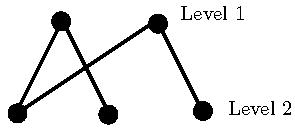
\includegraphics[width=0.5\textwidth]{random23}
\caption{A random bipartite graph $G'$.}\label{fig:random23}
\end{center}
\end{figure}


We now use $G'$ to build our routed network $G$
In order to create arcs with conflict, we add to each vertex of $G'$ an arc and a vertex in $G$. Let us call \textbf{conflict arcs} those arcs. The egdes of $E'$ becomes arcs of $A$, that we will call \textbf{core arcs}.

Figure~\ref{fig:extendnode} and figure~\ref{fig:extendendgraph} show how the first part of $G$ is built from $G'$.

\begin{minipage}{.5\linewidth}

\begin{center}
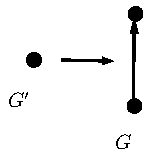
\includegraphics[width=0.4\textwidth]{extendnode}
\captionof{figure}{A node of $G'$ represent an arc in $G$.}\label{fig:extendnode}
\end{center}

\end{minipage}
\begin{minipage}{.5\linewidth}

\begin{center}
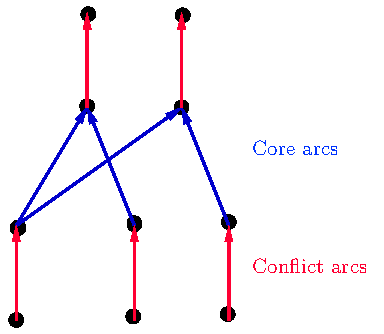
\includegraphics[width=0.4\textwidth]{extendendgraph}
\captionof{figure}{A node of $G'$ represent an arc in $G$.}\label{fig:extendendgraph}
\end{center}

\end{minipage}

 We now want to create some \textbf{final arcs}, that will model the last link before the antennas.
We generate $1\leq k\leq K$ final arcs before each contention arc $(u,v)$. We add $k$ new vertices $\{w_1,\ldots,w_k\}$ of indegree $0$ and outdegree $1$ to the set of vertices $V$. The new arcs $\{(w_1,u),\ldots,(w_k,u)\}$ are then added to $A$. 

Each route of the set of routes $\cal{R}$ of the routed network (G,$\cal{R}$) is composed either of one final arc and one contention arc (obtained from the set $S_1$ of arcs in $G'$), or one final arc, two contention arcs (one from $S_1$, one frome $S_2)$) and the core arc between those two contention arcs.
Note that one final arc belongs to one and only one route, while the core and contention arcs can be shared by several routes. 

Figure~\ref{fig:extendendgraph2} and figure~\ref{fig:extendendgraph3} shows how the final arcs are generated and define the routes of the routed network (G,$\cal{R}$). The routes of the same color share the same arcs after the final arc.

\begin{minipage}{.5\linewidth}

\begin{center}
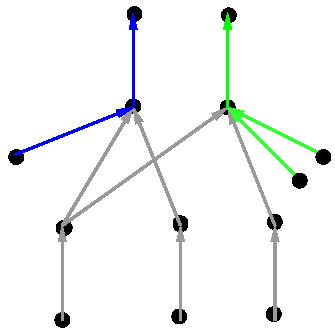
\includegraphics[width=0.4\linewidth]{extendendgraph2}
\captionof{figure}{Final arcs before contention arcs obtained from $S_1$.}\label{fig:extendendgraph2}
\end{center}

\end{minipage}
\begin{minipage}{.5\linewidth}
\begin{center}
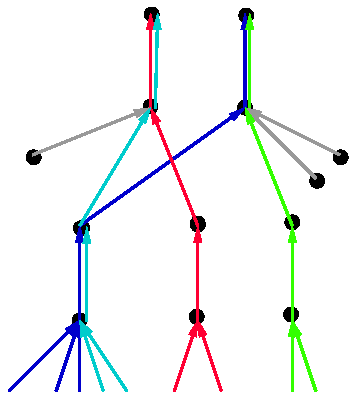
\includegraphics[width=0.4\linewidth]{extendendgraph3}
\captionof{figure}{Final arcs before contention arcs obtained from $S_2$.}\label{fig:extendendgraph3}
\end{center}
\end{minipage}
  The obtained routed network (G,$\cal{R}$) models a meshed network. The vertices of indegree $0$ of final arcs represent the antennas, the contention arcs from $S_1$ represent the last link before the datacenters, and the other nodes and arcs of the graph represent some links and switch of the network. This model seems to be close to realistic networks, but it is very difficult to obtain some sources of real topology.
  Figure~\ref{fig:extendendgraphgrey} shows the shape of the network modelized.

\begin{figure}[h]
\begin{center}
 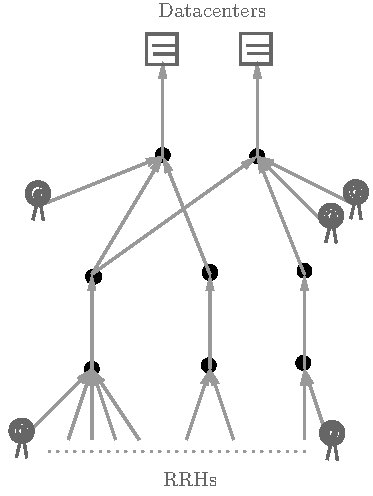
\includegraphics[width=0.4\textwidth]{extendendgraphgrey}
\caption{A network represented by a graph $G$.}\label{fig:extendendgraphgrey}
\end{center}
\end{figure}
    \end{subsection}

  \begin{subsection}{Implemented algorithms}
  
 

  The presented algorithm are designed to solve either problem PAZL or PALL.
  A \textbf{partial assignment}, is a set of departure times and waiting times $\{(\theta_0,w_0),\ldots,(\theta_k,w_k)\}$ with $k<n$, where $n$ is the number of routes in the network.
  
   
   
  In most of the presented algorithm, the following subroutine is used. Given a route $r$, a departure time $\theta_r$, a partial assignment of the routed network, and a way of the message, it returns $1$ if the message sent at time $\theta_r$ (if the way is forward) or $\theta_{\rho_r}$ (if the way is backward)  does not collide with the other messages. 
   	\begin{algorithm}[H]
 	\caption{MessageNoCollisions}
	\label{algo:messagenocollisions}
 	\begin{algorithmic}
 	\REQUIRE A route $r$, a departure time, and a way of the message (FORWARD/BACKWARD).
	\ENSURE $1$ if the messages can use the route with the given departure time and without collisions, $0$ otherwise.

 	\FORALL{Arcs in the route}
 	\IF{ There is a collision with the previous scheduled messages}
 	\STATE return $0$
 	\ENDIF
 	\ENDFOR
	\STATE return $1$
 	\end{algorithmic}
 	\end{algorithm}
 	
  \begin{subsubsection}{Algorithm to solve PAZL }

 Let $\frac{n\tau}{P}$ be the \textbf{load} of an arc. The load is the proportion of time slots used by the messages on the arc in a period. Therefore if the load is larger than $1$ there cannot be an assignment. We propose a greedy algorithm to build a $(P,\tau)$-periodic assignment, which always finds an assignment when the load is less than $1/4$.
 
 
 
 The period in an arc represent the behaviour of the traffic in the first tic of this arc, during a time of $P$ tics.
    
    \begin{proposition}
    There is a $(P,\tau)$-periodic assignment of a star routed network with waiting times $0$ if the load is less than $1/4$.
    \end{proposition}
    \begin{proof}
    The algorithm works by choosing an offset for each route in the following way: try all offsets in the period in the first arc of the route. Since the choice of an offset also sets the position of the message in the periods in the other arcs of the route forward and backward (because the waiting time is set to $0$), chose the first one which does not create a collision with the routes previously scheduled. We now prove that this algorithm always finds a $(P,\tau)$-periodic assignment without waiting time when $P \geq 4n\tau$ that is the load is less than $1/4$.
     
     We prove the previous property by induction on the number of routes: 
     Assume we are choosing the offset of the route $r_{k+1}$.
      Since the routing is coherent, two routes collides on a path, and if they are not in conflict on any arc of this path, they are not on the whole path.
     In the worst case, the $k+1^{th}$ route collides with the $k$ already scheduled routes in both ways, forward and backward. Thus, there is an arc in which all the $k$ collides. Consider the period on this arc, each of the $k$ datagram in this period prohibit $2\tau-1$ tics for the new routes; the $\tau$ tics of the datagram, and $\tau -1$ tics before the datagram. This means that, in the worst case, the $k$ datagram uses $(2\tau -1) \times k$ tics in this period.
     
     Remember that we try to chose the departure time in the first node of the $k+1^{th}$ route. Choosing an offset such there is no collisions with the other routes in the first arc of the route correspond to choose it in the arc in which the $k$ routes collides.
     
     Furthermore, since the routes can split between the way forward and backward, a datagram on the way backward can prohibit again $2\tau -1$ tics in the first node of the route. Thus, each of the $k$ previously scheduled datagrams can intersect with $(2\tau -1) \times k$ tics.
     This means that there is at most $4.k.\tau -2.k$ forbidden tics the first period of the route. Remember that $P \geq 4n\tau$, that mean we have at least $4n\tau$ tics in the forward period, and $k \leq n$. Thus $4n - 4k \geq 1$, which proves that the algorithm terminates and find a  $(P,\tau)$-periodic assignment. 
   
   
     \end{proof}
   
  \begin{paragraph}{Greedy Prime}
  The basic idea is to try to schedule the routes one by one. The routes are selected by id.  Then, given a route, we set the departure time for the datagram at the beginning of the route to $0$. If there is no collisions with the other routes, we give this departure time to the route. Otherwise, we increase the departure time of $1$ and call the Algorithm~\ref{algo:messagenocollisions} again, until we get a departure date that allows the datagram to pass the arcs without collisions with the routes already scheduled.

   	\begin{algorithm}[H]
 	\caption{Greedy Prime}
	\label{algo:greedyprime}
 	\begin{algorithmic}
 	\REQUIRE A graph, a set of routes, a period $P$
	\ENSURE A P-periodic assignment in p $\leq P$, or FAILURE

 	\FORALL{routes $i$ }
	\STATE date = $0$
	
 	\WHILE{!MessageCollisions($i$,date,FORWARD) $||$ !MessageCollisions($i$,date+routeLength($i$),BACKWARD) }
 	
 	\STATE date++;
 	\IF{date$ > P$}
	\STATE return FAILURE
	\ENDIF
 	\ENDWHILE
	\STATE DepartureDate($i$) = date;
 	\ENDFOR
	\STATE return departureDate
 	\end{algorithmic}
 	\end{algorithm}
 	The complexity of this algorithm is $\mathcal{O}(n\times P)$, with $n$ the number of routes and $P$ the period. It is very bad, since it depends of the period.
 	
 	  \end{paragraph}
    \begin{paragraph}{Swap}
    We propose an improvement of the Algorithm~.\ref{algo:greedyprime}: When there is no offset such that there is no collisions for a route $i$, we do the following:
    \begin{enumerate}
     \item Try an offset $o$ (for $0$ to $P-1$)
     \item Remove the routes which collide with this the new route $i$ for this offset (forward and backward way), and put it in a list.
     \item Assign the offset $o$ to $i$.
     \item Try to reschedule all the routes of the list
     \begin{itemize}
      \item If sucess : go back to the greedy prime routine.
      \item If failure : reassign the routes of the list to their original offset, and go back to step 1. 
     \end{itemize}
    \item If the route $i$ is still not scheduled, return failure.
    \end{enumerate}

    
  \end{paragraph}
    \begin{paragraph}{Greedy Min}
  
  We now try a smarter greedy algorithm.
   This algorithm helps us to pack the message in the arcs, indeed, if two message are spaced of a size $s < \tau$, those $s$ tics will be definitely lost since we can not use them to send a message. Thus, the idea is to pack as much as possible the messages on every arcs.
   We still take the routes one by one, sorted by id. Then, we try all departure times in the period. To each departure time is associated a "tic win" score, computed as follow : Considering a departure time that allow the datagram to pass the network without collisions, for each arc, we evaluate how much the new message is close to the other ones. We look $\tau$ tics before (and after) the message, and if there is another message scheduled at tic $i$ in the period, we increase the tic win score to $\tau -i$.
  The sum of the tic won score on each arc correspond to the tic won score of the departure time. We then assign to the route the departure time with the maximal tic won score.
 
  
 
    	\begin{algorithm}[H]
 	\caption{ticsWin}
	\label{algo:ticswin}
 	\begin{algorithmic}
 	\REQUIRE A route $r$, a departure time $t$
	\ENSURE $-1$ if the message can not pass without collisions, the number of tics win otherwise
	\STATE tmp  $\leftarrow$ $0$
 	\FORALL{Arcs $j$ in the route (forward AND backward)}
 	\IF{ There is a collision with the previous scheduled messages}
 	\STATE return $-1$
	\ELSE
	\STATE tmp += numberOfTicsWon(t,j)
 	\ENDIF
 	\ENDFOR
	\STATE return tmp
 	\end{algorithmic}
 	\end{algorithm}

	
   	\begin{algorithm}[H]
 	\caption{Greedy tics won}
 	\begin{algorithmic}
 	\REQUIRE A graph, a set of routes of size $n$, a period $P$
	\ENSURE A P-periodic assignment in p $\leq P$, or FAILURE

 	\FORALL{routes $i \in [0;n[$ }
	\STATE maxTicsWin $\leftarrow$ $-1$
	\STATE bestDepartureTime = $-1$
	\STATE departureTime[$n$]
	\FORALL{ offset $j \in [0;P[$ }
	\STATE tmp = ticsWin($r$,$j\times\tau$)
	\IF{  tmp  > maxTicsWin}
	\STATE maxTicsWin  $\leftarrow$ tmp
	\STATE bestDepartureTime  $\leftarrow$ $j$
	\ENDIF
 	\ENDFOR
	\IF{bestDepartureTime = $-1$}
	\STATE return FAILURE
	\ENDIF
	\STATE departureTime($i$) = $j\time\tau$
 	\ENDFOR
	\STATE return departureTime

 	\end{algorithmic}
 	\end{algorithm}
	
	The complexity of this algorithm is $\mathcal{O}(n\times P)$, with $n$ the number of routes and $P$ the period. Unlike the previous algorithm, the worst and medium complexity is the same, since we look at every departure times in the period.
\end{paragraph}
  \end{subsubsection}
    \begin{subsubsection}{Algorithms to solve PALL}
     We now allow the messages to be buffered in the BBUs. Thus have to choose the departure times and the waiting times of the datagrams.     
      \begin{paragraph}{Greedy Deadline}
      We choose to manage the routes in two steps.
      First, we send the datagrams in the way forward (from RRH to BBU).
      This part of the algorithm is basic and uses the same routine than the Algorithm:~\ref{algo:greedyprime}, the Greedy Prime algorithm. We take the route one by one, sorted by id, and we give for each route the first departure time that allow the datagram to reach the BBU without collisions. Note that we only check the way forward.
      
      Once we have scheduled the messages in the way forward, we want to send the answers. Consider that $u$ is the last vertex of the route forward (and so, the first of the route backward), the first step of the algorithm has fixed $t(d,u,r)$, that is, the time at which the datagram sent from the RRH has reach the node $u$. For each route, we compute $deadline(i) = Tmax - 2\times\lambda(i) - DepartureTime(i)$. This deadline can be seen as a budget: the lowest the deadline will be, the less waiting time is allowed on the route.\newline
      We the send the routes with the lowest deadline first in the way backward, trying all waiting times, starting to $0$, until the message can reach the RRH without collisions.
            
        \end{paragraph}

    \begin{paragraph}{Greedy Loaded}

In this algorithm, we choose to first take care of the most critical contention points first. Thus, we sort the arcs of the graph for the one in which there is the greater number of routes to the one in which there is the lower number of routes. Then we take first the more loaded link and we schedule the routes on it in two steps.
First, we search the lowest departure time such that there is no collisions in the way forward, then we do it again on the way backward. 

   	\begin{algorithm}[H]
 	\caption{Greedy Loaded}
 	\begin{algorithmic}
 	\REQUIRE A graph, a set of routes, a period $P$
	\ENSURE A P-periodic assignment

 	\FORALL{arcs $i$ sorted by decreasing number of routes using $i$}
	
 	\FORALL{ route $j$ on $i$}
	\IF{$j$ has not been scheduled yet}
	\STATE depTime = $0$
	
 	\WHILE{!MessageCollisions($j$,depTime,FORWARD) }
 	
 	\STATE depTime++;
 	\IF{depTime$ > P$}
	\STATE return FAILURE
	\ENDIF
 	\ENDWHILE
	\STATE DepartureTime($j$) = depTime;
	\STATE beginBackTime = depTime + routeLength($j$);
	\STATE backTime = beginBackTime;
	
 	\WHILE{!MessageCollisions($j$,backTime,BACKWARD) }
 	
 	\STATE tmp++;
 	\IF{backTime$ > P+beginBackTime$}
	\STATE return FAILURE
	\ENDIF
 	\ENDWHILE
	\STATE waitingTime($j$) = backTime-beginBackTime;
	\ENDIF
 	\ENDFOR

 	\ENDFOR
	\STATE return departureTime, waitingTime

 	\end{algorithmic}
 	\end{algorithm}
We also propose $3$ different orders to treat the route on the arcs. 
\begin{itemize}
\item By id.
\item From the longest to the shortest route.
\item By the number of collisions with the other routes on the entire network.
\end{itemize}
    \end{paragraph}
     	  \end{subsubsection}
  \begin{subsubsection}{Algorithm to solve \spall in the star}
  \todo{c'est ici mais ca ne parle pas de conflict depth 2}
  As mentioned in Lemma~\ref{lemma:spallorder}, reducing the waiting time to $0$ for the problem \spall does not have sense. Indeed, the departure time is already some waiting time, and we can transfer a part of this time to buffers in BBU, that allows us to consider only the sending order of the route on the way forward.
  \begin{theorem} In a star shaped network, $\spall  \in FPT$ when parameterized by the number of routes.
  \end{theorem}
\begin{proof}
As we just mentioned, for the way forward, it is enough to consider the sending order of the routes to capture all the solutions.
Since we already have an FPT algorithm that solves the way backward \cite{Guir1806:Deterministic}, we then apply it to each sending order.
\end{proof}

It is possible to reduce the complexity of the $n!$ sending orders on the way forward. Indeed, once a sending order is generated, it is easy to compute the deadline for all route and to determine if yes or no, the input will fail in our fpt algorithm for the backward way.
\todo{implémenter cette amélioration: en utilisant un branch and bound}


  \end{subsubsection}
\end{subsection}

\begin{subsection}{Compact representation}

We explain in this section how to represent an assignment for the problem 
\spall over an instance of depth $1$ in a compact way. Then, this representation
can be used at any contention point in an instance of larger depth.
Not all solutions can be represented in a compact way, but there
is at least one optimal assignment for \spall wich is.
It allows to design FPT algorithm by going through all compact 
representations. We obtain good heuristic algorithms using taboo search or simulated annealing, since one can easily define the neighborood of a compact representation.

\begin{definition}
A compact representation of an assignment over $n$ routes is a pair $(O,S)$,
where $O$ is an order on the $n$ routes and $S$ is a subset of the $n$ routes.
\end{definition}

We now explain how to decompress a compact representation into an assignment.
\todo{Je ne connais pas les notations pour \spall, je suppose qu'on a des temps
d'arrivée sur l'arc $a_1,\dots,a_n$ et qu'on fixe des temps de départ sur l'arc 
$d_1,\dots,d_n$. Je note un assignement A. Je remarque qu'on a souvent omis des 
fonctions comme PT, TR la dépendence en l'assignement, du coup certaines choses sont 
plus dures à écrire proprement}
Say w.l.o.g. that the routes are indexed in the order given by $O$.
We fix the departure of the first route $d_1 = a_1$, that is the packet of this route do not wait in a buffer. Then, in each period beginning by the first route, the routes will be in order. To simplify, we assume that $d_1 = a_1 = 0$, which can be obtained by removing $a_1$
to all arrival times. We fix the departure times of the route in order, when the first $i$ routes have their departure time computed, we fix $a_{i+1}$ in the following way. 

If $i+1 \notin S$, then $d_{i+1} >= a_{i+1}$ otherwise the route $i+1$ should go in the period after the one it is available in, that is $d_{i+1} > (a_{i+1}/P + 1)P$.
The value of  $d_{i+1}$ is the smallest value which satisfies the previous constraint,
ensures that there are no collision with the first $i$ routes and  satisfies the order, that is $d_{i+1} \mod P > d_i \mod P$. 
It is possible that the process fails to find a correct value for $d_i$ at some point,
in that case there are no assignment associated to this compact representation.

We denote this transformation by $Sol$, that is $Sol(O,S)$ is the solution previously defined
(the routed network is implicit) or a special value to denote there is no assignment compatible with this compact representation. 

We can also define an inverse function which from most assignment $A$ computes a compact representation, that we denote by $Compact(A)$. The function is define only for
assignments $A = (a_1,\dots,a_n)$, such that the first route has no waiting time, that is $a_1 = d_1$. Assume w.l.o.g that $a_1 = d_1 = 0$, by considering the equivalent problem where $a_i= a_i -a_1$ and $d_i = d_i - a_1$.
Compute the values $(d_i)\mod P$ and  call their order $O$. Let 
 $S$ be the set of $i$ such that $(d_i \geq (a_i / P + 1) P$. We let $Compact(A) = (O,S)$.


A compact representation of a solution for an instance of depth larger than $k$
is a list of compact representations, one for each contention arc. The following theorem explains why it is enough to explore the compact representations to solve \spall.

\begin{theorem}
Among all assignments for a routed network $G,{\cal R})$, there is a compact representation which minimizes $TR(G,{\cal R})$.
\end{theorem}
\begin{proof}
Idée, si on regarde un assignement et que toutes les routes d'un arc ont 
un temps d'attente alors on peut trouver une solution au moins aussi bonne ou 
une route n'attends pas. Ensuite on montre que pour un assignement A donné, 
Sol(Compact(A)) a un meilleur $TR(G,{\cal R})$. Tout a été défini pour ça, mais il faut le montrer.

\end{proof}
\end{subsection}
  

\end{section}
	 

\bibliographystyle{ieeetr}
\bibliography{srcs}
\end{document}
